\subsection{Universal Asynchronous Receiver Transmitter(UART)}
En UART er et led mellem et parallelt og serielt interface, der både modtager data(RX) og sender data(TX). Dataen sendes som bit, og kan både sendes serielt eller parallelt.\citep{Jimb02016a,Chun-zhiYin-shuiLun-yao2011}\newline 
Parallelt bliver flere bit overført på samme tid, hvormed et 8-bit system er nødsaget til at have 8 ledninger, hvor der i den ene ende er en RX kobling og den anden er TX kobling.\citep{Jimb02016a}\newline
Den serielle kommunikation foregår asynkront, og kan foregå med en ledning, da kun en bit overføres af gangen. Oftest benyttes den serielle kommunikation, da denne ikke kræver så mange ledninger.  Det er nødvendigt at sætte en baudrate, da TX sender i forhold til denne og RX sampler i forhold til den forventede baudrate\fxnote{baudrate = Hvor hurtigt der sendes data (bits per sekund[bps])}. Det modtagne data gemmes ofte i en buffer, som efterfølgende videregives i form af firs-in-first-out (FIFO) princippet.\citep{Jimb02016a}\newline 
Overførsel af data sker asynkront, som det ses på \figref{fig:asynkron}. Ved denne kommunikationsform opererer RX og TX ved to forskellige klokker. For at kunne lave dataen synkront, sættes der et startbit og et stopbit. UARTens opgave er at læse data fra FIFO parallel data, som så laves om til seriel data Dette data kan så sendes til andre enheder. Når RX i en anden enhed modtager et startbit, laves data om fra seriel til parallel data, hvorefter data kan skrives til modtager-FIFO.\citep{Jimb02016a,Chun-zhiYin-shuiLun-yao2011}

\begin{figure}[H]
	\centering
	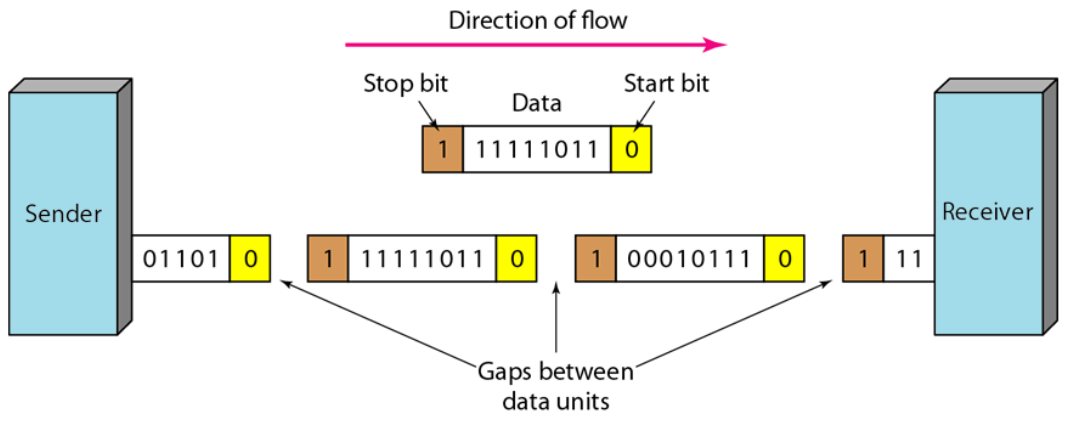
\includegraphics[scale=0.6]{figures/bProblemloesning/asynkron.png}
	\caption{På figuren ses asynkron dataoverførsel.\citep{Jimb02016}}
	\label{fig:asynkron}
\end{figure}

Nogle enheder indeholder mere end en seriel-linje, og disse enheder fungerer enten som fuld-duplex eller halv-duplex. De enheder der er fuld-duplex, kan både sende og modtage data på samme tid. Ved halv-duplex, skal dette foregå på skift.\citep{Jimb02016a,Chun-zhiYin-shuiLun-yao2011}